% !TeX program = pdflatex
\documentclass[tikz,border=8pt]{standalone}
\usepackage{tikz}
\definecolor{FigureBlue}{HTML}{2563EB}\definecolor{FigureOrange}{HTML}{EA580C}
\begin{document}
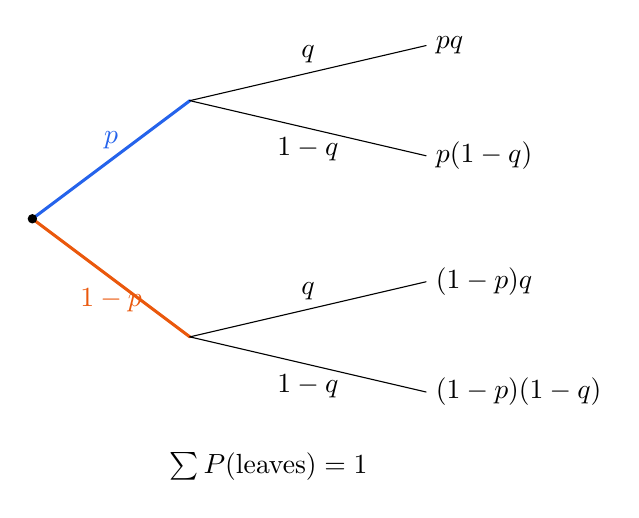
\begin{tikzpicture}[line cap=round]
  \coordinate (R) at (0,0); \coordinate (A) at (2,1.5); \coordinate (B) at (2,-1.5);
  \coordinate (AA) at (5,2.2); \coordinate (AB) at (5,.8); \coordinate (BA) at (5,-.8); \coordinate (BB) at (5,-2.2);
  \draw[FigureBlue,line width=1.1pt] (R)--(A) node[midway,above] {$p$}; \draw[FigureOrange,line width=1.1pt] (R)--(B) node[midway,below] {$1-p$};
  \draw (A)--(AA) node[midway,above] {$q$}; \draw (A)--(AB) node[midway,below] {$1-q$};
  \draw (B)--(BA) node[midway,above] {$q$}; \draw (B)--(BB) node[midway,below] {$1-q$};
  \node[right] at (AA) {$pq$}; \node[right] at (AB) {$p(1-q)$}; \node[right] at (BA) {$(1-p)q$}; \node[right] at (BB) {$(1-p)(1-q)$};
  \fill (R) circle (1.7pt); \node at (3,-3.15) {$\sum P(\mathrm{leaves})=1$};
\end{tikzpicture}
\end{document}
